\section{BACKGROUND}
\label{sec:background}

\subsection{NOTATIONS}
\label{subsec:notations}

We use bold lowercase letters to refer to vectors, such as $\rvr$, and bold capital letters to refer to matrices, like $\rmW$. non-bold lowercase letters are scalars. For example, $u_{i,r} \in \sR$ is the $r$th component of vector $\rvu_i \in \sR^m$. $\rvone$ means an all-one vector, and $\rmI$ refers to an identity matrix, with dimensions depend on the contexts.

In the sequel, $n$ is the total number of states, while $m$ is the total number of nodes in each hidden layer. $h$ is the total number of actions can be taken at each state.

Denote $[n] \triangleq \left\{ 1,2, \dots, n \right\}$. $\rvs_i \in \sR^d$, $i \in [n]$ refers to the feature vector of the $i$th state. $\rvw_r \in \sR^d$, $r \in [m]$ is a weight vector in the first hidden layer. $\rmW^\top \triangleq \left[ \rvw_1, \rvw_2, \dots, \rvw_m \right] \in \sR^{d \times m}$ is the weight matrix of the first hidden layer. $u_{i,r} \triangleq \rvw_r^\top \rvs_i$ is the $r$th node value of the first hidden layer. $\rva_k \in \sR^m$, $k \in [h]$ is a weight vector in the second hidden layer. $\rmA^\top \triangleq \left[ \rva_1, \rva_2, \dots, \rva_h \right] \in \sR^{m \times h}$ is the weight matrix of the second hidden layer. $o_{i,k} \triangleq \sum\limits_{r=1}^{m}{a_{k,r} \cdot \sigma\left( u_{i,r} \right)}$ is the logit of the $k$th action for state $\rvs_i$, where $\sigma(\cdot) \triangleq \max\left\{ \cdot, 0 \right\}$ is the ReLU activation function. $\pi_{i,k} \triangleq f\left( o_{i,k} \right) \triangleq \frac{\exp\left\{ o_{i,k} \right\}}{\sum\limits_{k^\prime = 1}^{h}{\exp\left\{ o_{i,k^\prime} \right\}}}$ is the probability of choosing action $k$ at state $\rvs_i$, where $f(\cdot)$ is the softmax function. $\rvr_i \in \sR^h$ is the true mean reward vector at state $\rvs_i$. $\rvpi_i^* \triangleq \argmax\limits_{\rvpi \in \Delta^{h-1}}{\left\{ \rvpi^\top \rvr_i \right\}}$ is the optimal policy at state $\rvs_i$. Given stochastic policies $\rvpi \triangleq \left[ \rvpi_1, \rvpi_2, \dots, \rvpi_n \right] \in \sR^{h \times n}$, the expected (mean) loss is defined as,
\begin{equation}
\label{eq:expected_loss}
\begin{split}
    \frac{1}{n} \cdot \sum\limits_{i=1}^{n}{ \left( {\rvpi_i^*}^\top \rvr_i - \rvpi_i^\top \rvr_i \right) }.
\end{split}
\end{equation}

Without loss of generality, we assume $\rvr_i \in \left[ 0, 1 \right]^h$, and $\rvr_i$ is the mean vector of some random reward vectors,  $\forall i \in [n]$.

\subsection{STOCHASTIC BANDIT SETTINGS}
\label{subsec:settings}

We mainly focus on the standard stochastic bandit setting with $n = 1$, i.e., there is only one state $\rvs_i$. At each time step $t$, the agent takes an action $A_t \in [h]$ according to its own strategies, and then it observes a random reward $R_{i, A_t} \in \sR$, where the mean value of $R_{i, A_t}$ is $r_{i, A_t}$. The agent then uses the reward to improve its action selection strategies. After such $T$ time steps, the performance of the agent's strategy is measured by the (expected) regret,
\begin{equation}
\label{eq:expected_regret}
    \sum\limits_{t=0}^{T-1}{{\rvpi_i^*}^\top \rvr_i} - \sE \left[ \sum\limits_{t=0}^{T-1}{  r_{i, A_t}  } \right] = \sum\limits_{t=0}^{T-1}{{\rvpi_i^*}^\top \rvr_i} - \sum\limits_{t=0}^{T-1}{ \sE \left[ r_{i, A_t} \right] },
\end{equation}
where the expectation is over the randomness of action selection, if the agent is using some stochastic strategies.

Although there is only one state, i.e., $n = 1$, and $i$ can be omitted without ambiguity, we choose to keep the subscript $i$ here to make the generalization from the standard bandit setting to the many state dependent setting smoother, and our algorithms work for general $n > 1$. For simplicity, we assume $\left\| \rvs_{i} \right\|_2 = 1$, $\forall i \in [n]$.

In the case of $n > 1$, for each state $\rvs_i$, there is a state dependent policy $\rvpi_i$. And the agent's goal is to learn totally $n$ policies using only one neural network. We assume $\left\| \rvs_{i} -  \rvs_{j} \right\|_2 \ge \delta > 0 , \ \forall i \not= j$, i.e., no duplicated data, and $\left\| \rvs_{i} \right\|_2 = 1, \ \forall i \in [n]$.

\subsubsection{Episodic Markov decision process (MDP) (maybe remove this section)}

The episodic MDP setting recovers the bandit setting as a special case. The environment randomly select a starting state $\rvs_i^0 \in \sR^d$. At each time step $t$, the agent takes one action $A_t \in [h]$ according to some strategies, and then it observes a reward $R_{i, A_t} \in \sR$ and next state $S_{t+1} \sim \sP\left( \cdot \middle| S_t, A_t \right)$, where $\sP$ is the transition probability matrix and it is unknown to the agent. After such $H$ steps, the agent observes an ending state $S_H$, and the current trajectory terminates. At the next time step, the agent will observe a new starting state $\rvs_i^0$ randomly generated by the environment. Since we use policy gradient method (no value learning), the agent updates its NN policy weights using the cumulative reward collected after each single trajectory terminates.

\begin{figure}[t]
\vskip 0.2in
\begin{center}
\centerline{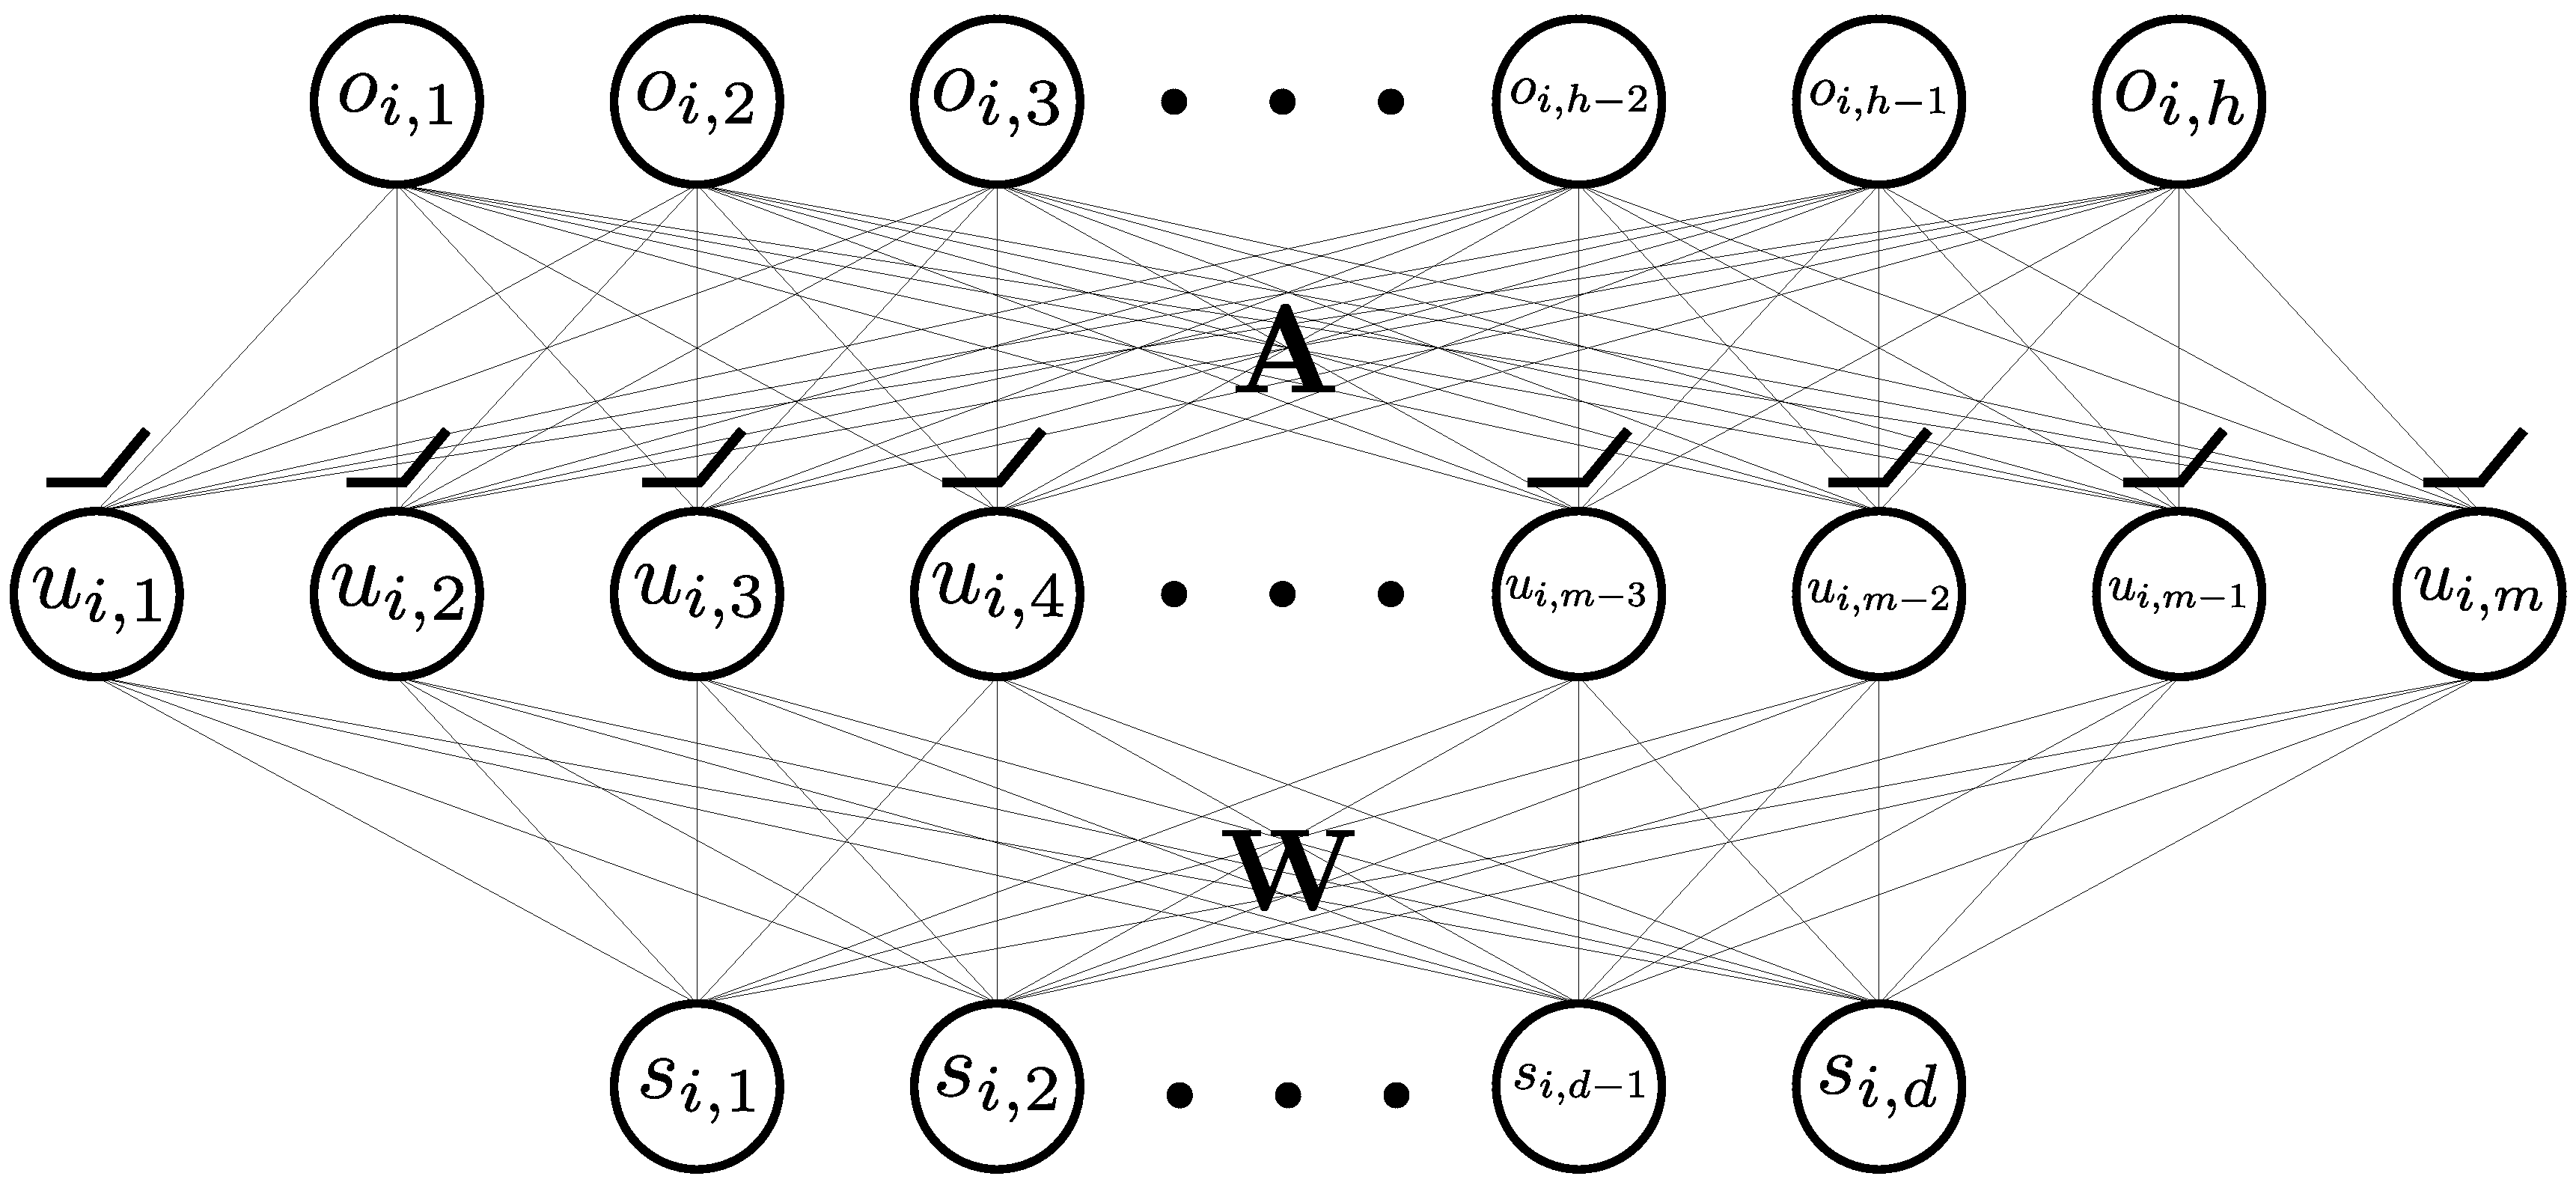
\includegraphics[width=\columnwidth]{nn_value.pdf}}
\caption{Value neural network.}
\label{fig:nn_value}
\end{center}
\vskip -0.2in
\end{figure}

\subsection{NEURAL NETWORK VALUE FUNCTION APPROXIMATION AND POLICY}
\label{subsec:nn_policy}

The structures of the two layer value and policy neural network with ReLU activation are shown in \cref{fig:nn_value} and \cref{fig:nn_policy}, respectively. The policy neural network differs the value neural network with one additional softmax transform layer, in order to output probability distributions. 

Both the value and the policy neural networks take the state feature  $\rvs_i \in \sR^d$ as the input. Then the networks calculate the hidden node value vector by $u_{i,r} \triangleq \rvw_r^\top \rvs_i$, $\forall r \in [m]$. The logit vector is then calculated by $o_{i,k} \triangleq \rva_k^\top \sigma\left( \rvu_i \right)$, $\forall k \in [h]$, where $\sigma$ is element-wise ReLU activation function. The value neural network outputs the logit vector $\rvo_i$. While the policy neural network output probability is the softmax transform of the logit vector, i.e., $\rvpi_i \triangleq f\left( \rvo_i \right) = f\left( \rmA \sigma\left( \rmW \rvs_i \right) \right)$. 

\begin{figure}[t]
\vskip 0.2in
\begin{center}
\centerline{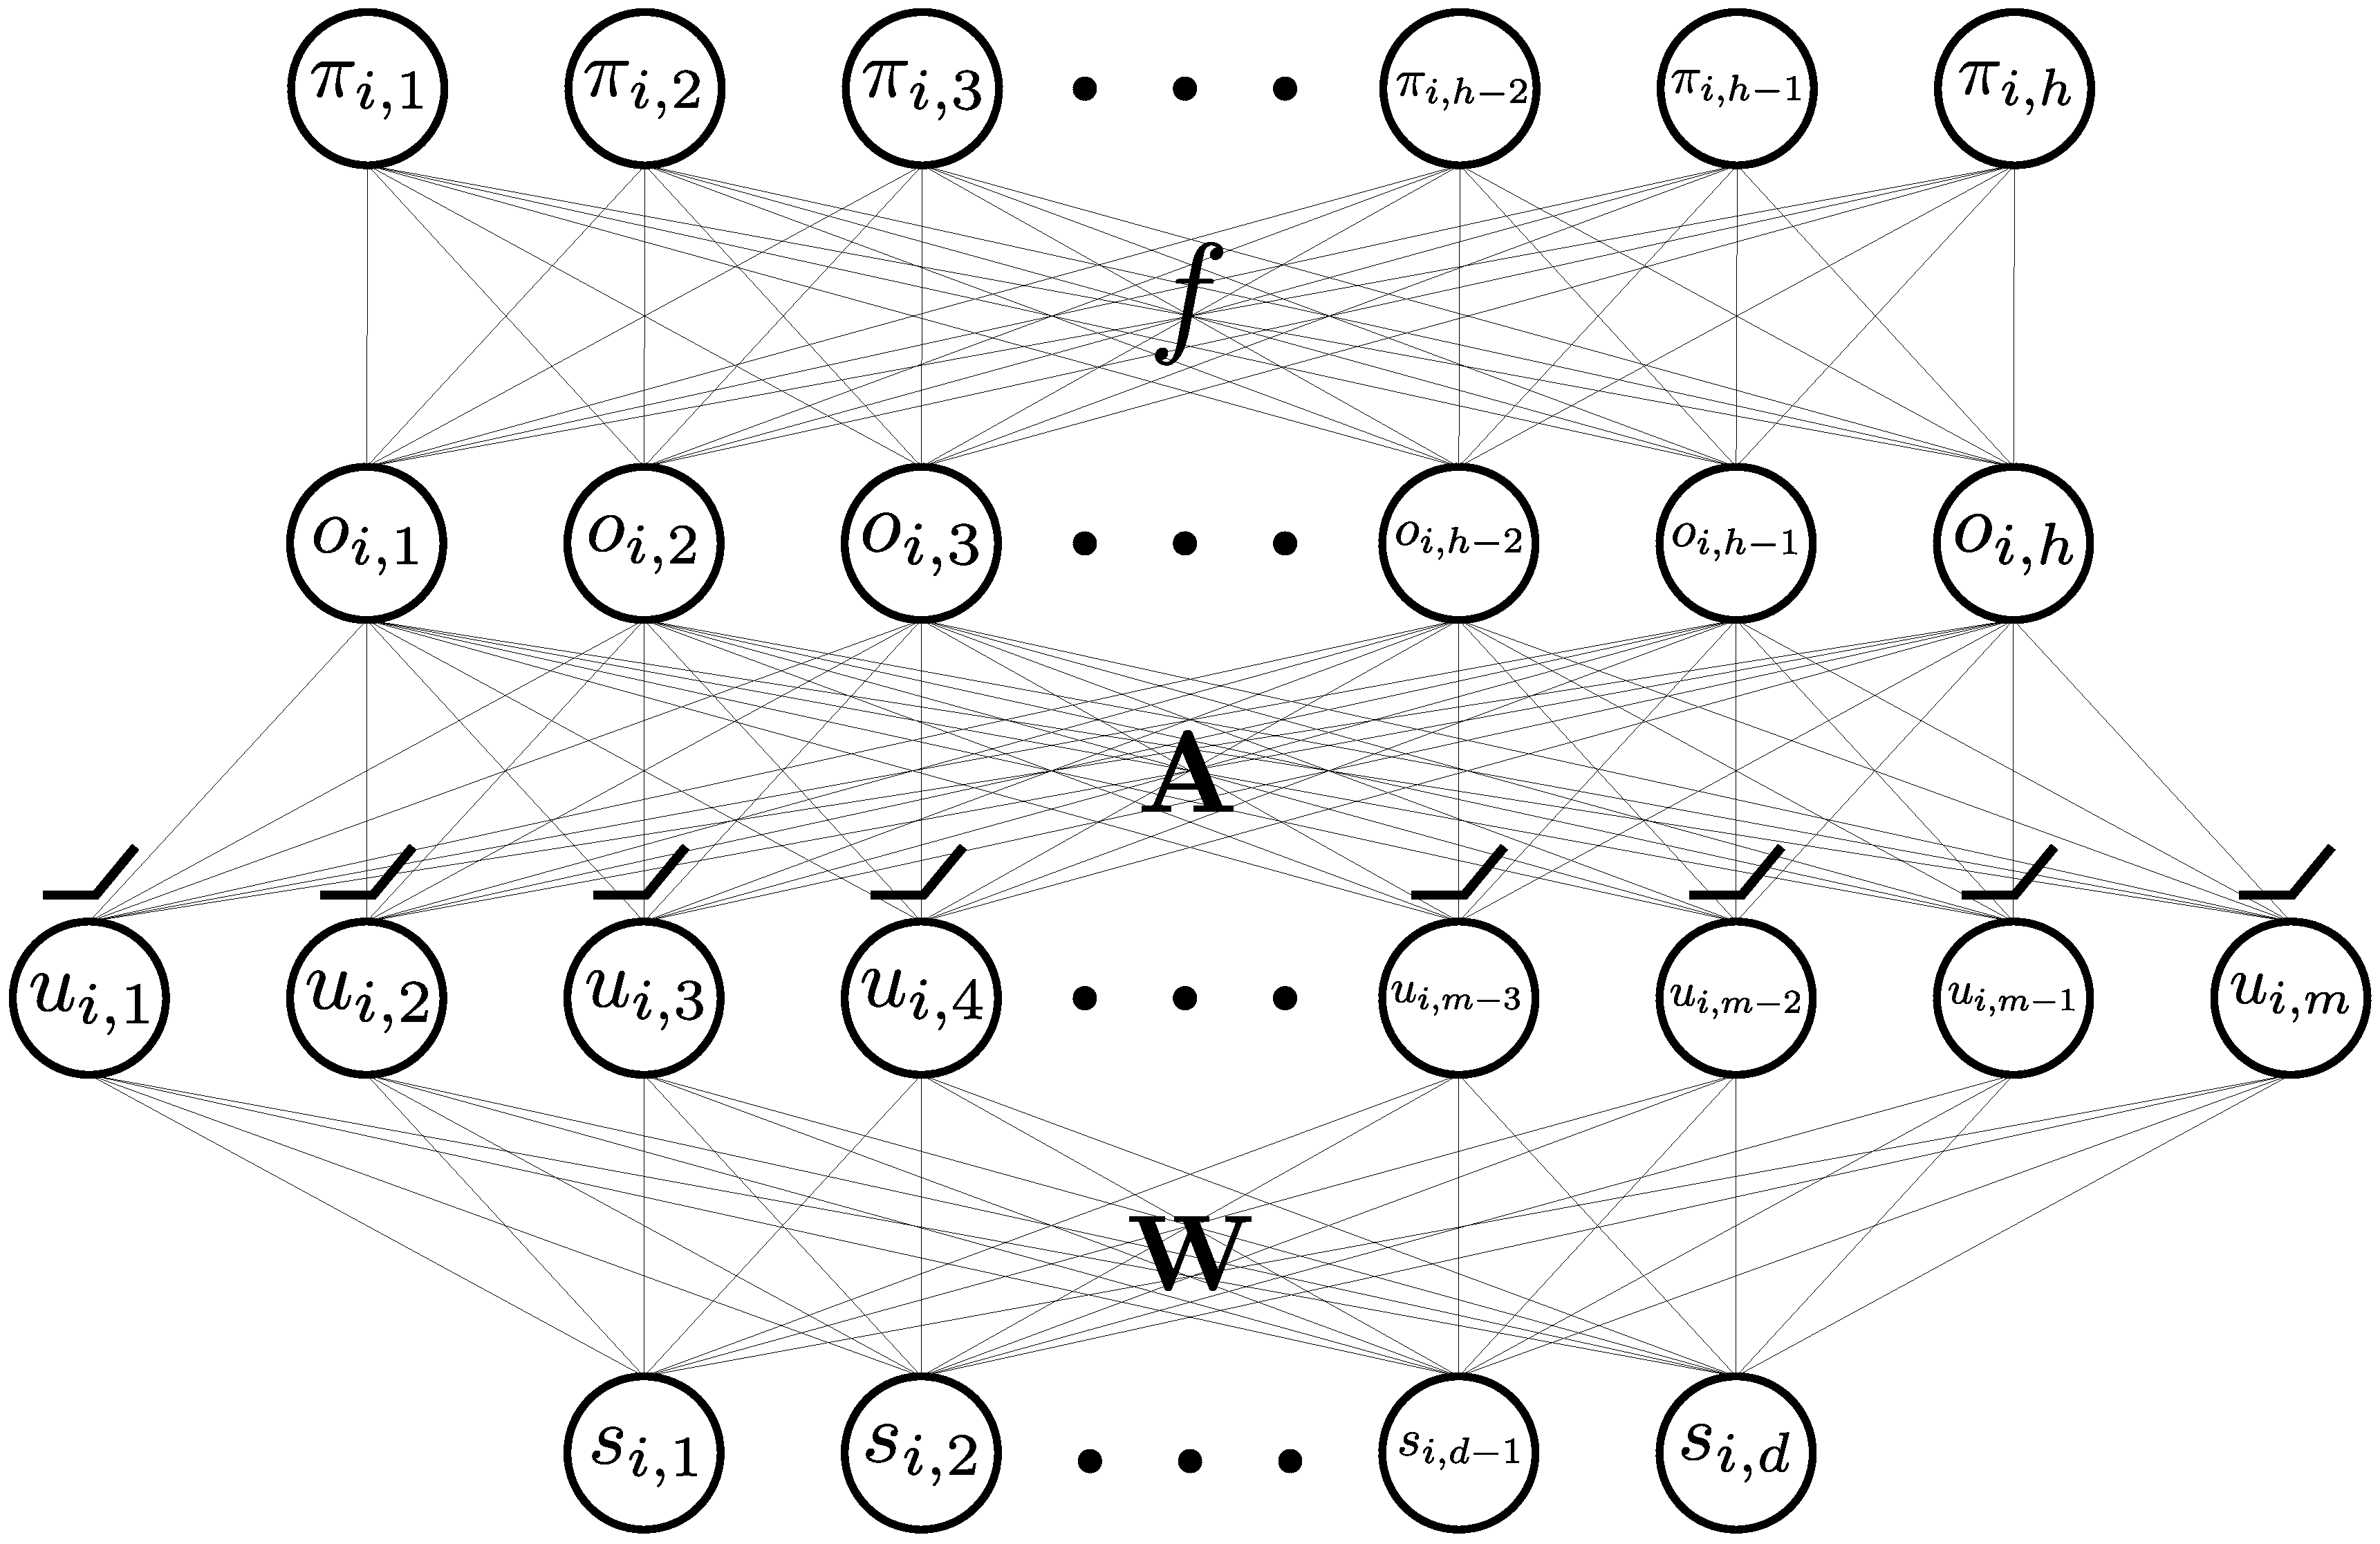
\includegraphics[width=\columnwidth]{nn_policy.pdf}}
\caption{Policy neural network.}
\label{fig:nn_policy}
\end{center}
\vskip -0.2in
\end{figure}

The policy neural network defines a family of policies $\rvpi_i \left( \rmW \right)$ parameterized by $\rmW \in \sR^{m \times d}$ given any state $\rvs_i$. Let $\rvpi_i = \rvpi_i \left( \rmW \right)$, the expected loss of the policy neural network can be calculated according to \cref{eq:expected_loss}.

We would like to point that our algorithms work for general value functions and policies parameterized by multi-layered neural networks \citep{allen2018convergenceA,allen2018convergenceB,du2018gradientA}. Using two layer neural networks here is just for simplicity and conciseness.

\subsection{LOGIT LEARNING}
\label{subsec:logit_learning}

Our first proposed algorithm is Logit Learning with $\epsilon$-Greedy Exploration, as shown in \cref{alg:logit_learning_eps_greedy_exploration}. After the random initialization, at each time step $t$, the agent selects the action with the largest logit with probability $1 - \epsilon_t$, and it uniformly randomly select actions with the other probability $\epsilon_t$. After taking action and observing rewards, the agent improves its strategies by minimizing the value loss objective $\frac{1}{2} \left\| \rvo\left( \rmW\left(t\right)\right) - \hat{\rvr}_i\left(t\right) \right\|_2^2$, where $\hat{\rvr}_i\left(t\right)$ is the empirical estimation from sampled rewards up to step $t$. In each iteration, the agent only update its value neural network using one gradient descent, therefore the logit learning is in an online fashion.


\begin{algorithm}[h]
   \caption{Logit Learning with $\epsilon$-Greedy Exploration}
\label{alg:logit_learning_eps_greedy_exploration}
\begin{algorithmic}
   \STATE {\bfseries Input:} State feature $\rvs_i$, learning rate $\eta > 0$.
   \STATE $\rvw_r(0) \sim \gN\left( 0, \sigma^2 \cdot \rmI \right)$, $\forall r \in [m]$.
   \STATE $a_{k, r} \sim \gU\left\{-1, +1\right\}$, $\forall k \in [h]$, $\forall r \in [m]$.
   \STATE $\hat{r}_{i,k}\left(0\right) \gets 0$, $n_{i,k}\left(0\right) \gets 0$, $\forall k \in [h]$.
   \STATE $\hat{\Delta}_{i,k}\left(0\right) \gets \max\limits_{k^\prime}\left\{ \hat{r}_{i,k^\prime}\left(0\right) \right\} - \hat{r}_{i,k}\left(0\right)$, $\forall k \in [h]$.
   \STATE $\tilde{\Delta}_{i,k}\left(0\right) \gets \max\limits_{k^\prime}\left\{ o_{i,k^\prime}\left(0\right) \right\} - o_{i,k}\left(0\right)$, $\forall k \in [h]$.
   \FOR{$t=0$ {\bfseries to} $T-1$}
   \STATE $\xi_t \gets \frac{\log{t}}{t \hat{\Delta}_{i,k}^2\left(0\right)}$, $\epsilon_t \gets \min\left\{ \frac{1}{2 h}, \xi_t \right\}$.
   \STATE $\rvpi_i\left(t\right) \gets \frac{ \exp\left\{ \frac{ \rvo\left( \rmW\left(t\right)\right) }{\tau} \right\} }{\rvone^\top \exp\left\{ \frac{ \rvo\left( \rmW\left(t\right)\right) }{\tau} \right\} } $.
   \STATE $\tilde{\rvpi}_i\left(t\right) \gets \left( 1 - \epsilon_t \right) \cdot  \rvpi_i\left(t\right) + \epsilon_t \cdot \gU{\left[ h \right]}$.
   \STATE Sample action $A_{t} \sim \tilde{\rvpi}_{i}\left(t\right)\left(\cdot \middle| \rvs_i \right)$.
   \STATE Take action $A_{t}$. Observe reward $R_{i, A_{t}}\left(n_{i, A_{t}}\left(t\right) \right)$.
   \STATE $n_{i, A_{t}}\left(t+1\right) \gets n_{i, A_{t}}\left(t\right) + 1$.
   \STATE $\hat{r}_{i,A_{t}}\left(t+1\right) \gets \frac{n_{i, A_{t}}\left(t\right) \cdot \hat{r}_{i,A_{t}}\left(t\right) + R_{i, A_{t}}\left(n_{i, A_{t}}\left(t\right)\right) }{n_{i, A_{t}}\left(t+1\right)}$.
   \STATE $n_{i, k}\left(t+1\right) \gets n_{i, k}\left(t\right)$, $\forall k \not= A_t$.
   \STATE $\hat{r}_{i,k}\left(t+1\right) \gets \hat{r}_{i,k}\left(t\right)$, $\forall k \not= A_t$.
   \STATE $\rmW(t+1) \leftarrow \rmW(t) - \eta \cdot \frac{d \left\{ \frac{1}{2} \left\| \rvo\left( \rmW\left(t\right)\right) - \hat{\rvr}_i\left(t\right) \right\|_2^2 \right\}}{d \rmW(t)}$.
   \ENDFOR
\end{algorithmic}
\end{algorithm}

uai2019================

\subsection{VANILLA POLICY GRADIENT}
\label{subsec:vanilla_policy_gradient}

During interacting with the environment, the agent can use any strategies to select actions. In particular, if at each time step $t$, the agent's action selection strategy is the NN policy $\rvpi_i\left(\rmW(t)\right)$, then the (expected) regret is equivalent to the cumulative expected loss of $\rvpi_i\left(\rmW(t)\right)$, i.e., 
\begin{equation}
\label{eq:vanilla_policy_gradient_expected_regret}
\begin{split}
    &\sum\limits_{t=0}^{T-1}{{\rvpi_i^*}^\top \rvr_i} - \sum\limits_{t=0}^{T-1}{ \expectation\limits_{A_t \sim \rvpi_i\left(\rmW(t)\right)} \left[ r_{i, A_t} \right] } \\
    &= \sum\limits_{t=0}^{T-1}{{\rvpi_i^*}^\top \rvr_i} - \sum\limits_{t=0}^{T-1}{\rvpi_i\left(\rmW(t)\right)^\top \rvr_i},
\end{split}
\end{equation}
according to \cref{eq:expected_loss} and \cref{eq:expected_regret}. Using \cref{eq:vanilla_policy_gradient_expected_regret}, at each time step $t$, the agent can use the current NN policy $\rvpi_i\left(\rmW(t)\right)$ to sample an action, and obtain an estimation of the expected loss $\rvpi_i\left(\rmW(t)\right)^\top \rvr_i$. Doing policy gradient updates with respect to the NN weights $\rmW(t)$ will arguably decrease the expected loss, thus reduce the expected regret. 

However, the above mentioned method, called as vanilla policy gradient, often suffers the ``lack of exploration" problem in practice, i.e., some actions can never be explored thus cannot be learned. Unfortunately, without any other techniques, the vanilla policy gradient method cannot avoid this issue. Actually, as our analysis shown later on, the convergence rate of the policy expected loss relies on non-zero probability of exploring the optimal arms, which is consistent with intuition. For this reason, we need mix the vanilla policy gradient method with explicit exploration.

\subsection{POLICY GRADIENT WITH UNIFORM EXPLORATION}
\label{subsec:policy_gradient_with_uniform_exploration}

Our proposed algorithm adds explicit uniform exploration to the vanilla policy gradient method, as shown in \cref{alg:policy_gradient_uniform_exploration}. After the random initialization, at each time step $t$, one of the two cases happens. If $t < T^{\frac{2}{3} + \beta}$, then agent gets into a purely ``exploring phase", without learning the policy NN, while just collecting empirically estimated rewards. If $t \ge T^{\frac{2}{3} + \beta}$, then the agent starts ``playing and learning". The agent samples and takes actions according to the current NN policy $\rvpi_{i}\left(\rmW(t)\right)$. In the meanwhile, the agent learn the NN policy by doing policy gradient updates, with the expected empirically estimated loss calculated from the exploring phase as its objective.

\begin{algorithm}[t]
   \caption{NN Policy Gradient with Uniform Exploration}
\label{alg:policy_gradient_uniform_exploration}
\begin{algorithmic}
   \STATE {\bfseries Input:} State feature $\rvs_i$, learning rate $\eta > 0$, $\beta > 0$.
   \STATE Initialize $\rvw_r(0) \sim \gN\left( 0, \sigma^2 \cdot \rmI \right)$, $\forall r \in [m]$. \STATE Initialize $a_{k, r} \sim \gU\left\{-1, +1\right\}$, $\forall k \in [h]$, $\forall r \in [m]$.
   \STATE Initialize $\hat{r}_{i,k}\left(0\right) \gets 0$, $n_{i,k}\left(0\right) \gets 0$, $\forall k \in [h]$.
   \FOR{$t=0$ {\bfseries to} $T-1$}
   \IF{$t < T^{\frac{2}{3} + \beta}$}
   \STATE (Exploring Phase)
   \STATE $\rmW(t+1) \leftarrow \rmW(t)$.
   \STATE Uniformly randomly sample action $A_{t} \in [h]$.
   \ELSE
   \STATE (Playing-Learning Phase)
   \STATE $\rmW(t+1) \leftarrow \rmW(t) + \eta \cdot \frac{d \rvpi_{i}\left(\rmW(t)\right)^\top \hat{\rvr}_i \left(t\right)}{d \rmW(t)}$.
   \STATE Sample action $A_{t} \sim \rvpi_{i}\left(\rmW(t)\right)\left(\cdot \middle| \rvs_i \right)$.
   \ENDIF
   \STATE Take action $A_{t}$. Observe reward $R_{i, A_{t}}\left(n_{i, A_{t}}\left(t\right) \right)$.
   \STATE $n_{i, A_{t}}\left(t+1\right) \gets n_{i, A_{t}}\left(t\right) + 1$.
   \STATE $\hat{r}_{i,A_{t}}\left(t+1\right) \gets \frac{n_{i, A_{t}}\left(t\right) \cdot \hat{r}_{i,A_{t}}\left(t\right) + R_{i, A_{t}}\left(n_{i, A_{t}}\left(t\right)\right) }{n_{i, A_{t}}\left(t+1\right)}$.
   \STATE $n_{i, k}\left(t+1\right) \gets n_{i, k}\left(t\right)$, $\forall k \not= A_t$.
   \STATE $\hat{r}_{i,k}\left(t+1\right) \gets \hat{r}_{i,k}\left(t\right)$, $\forall k \not= A_t$.
   \ENDFOR
\end{algorithmic}
\end{algorithm}

Note in \cref{alg:policy_gradient_uniform_exploration}, after the random initialization $a_{k,r} \sim \gU\left\{-1, +1\right\}$, $a_{k,r}$ is fixed, which is common in literature \citep{li2018learning,du2018gradientA,du2018gradientB,allen2018convergenceA,allen2018convergenceB}, and empirically verified that has no impact on the performance of trained NNs \citep{hoffer2018fix}. Other initialization like $\rva_k \sim \gN(0, \rmI)$ also works.


